A simulação foi realizada no software RoboDK, software offline utilizado para simulação de robôs industriais. Para realização da simulação foram utilizados as posições escolhidas na análise dimensional. Ao se comparar os resultados de $T_\mathrm{home}$ e $T_\mathrm{escolhido}$, é possível comprovar que a matriz T representa o modelo cinemático do robô.

Para comprovar o explicito acima, inicialmente, analisa-se a posição do modelo em \textit{home}, como indicado na FIG. \ref{fig:home_simulacao}.

\begin{figure}[ht]
    \centering
    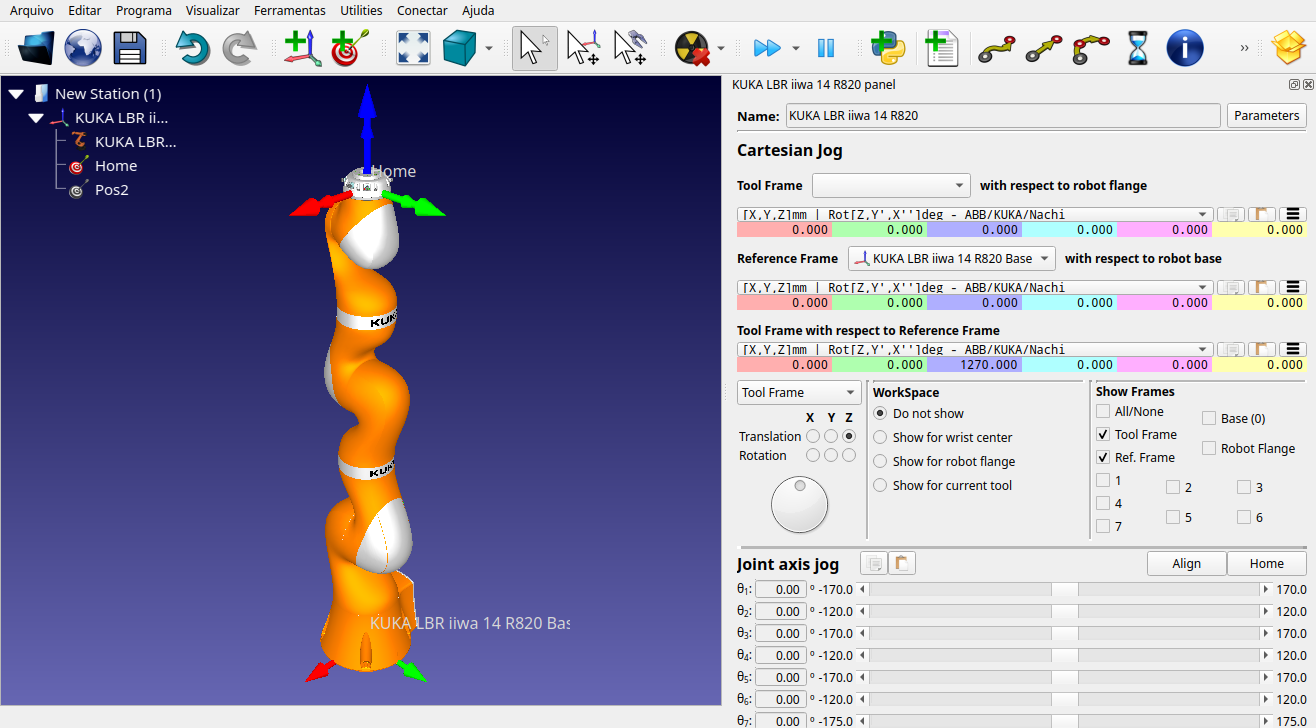
\includegraphics[scale=0.25]{Imagem/home.png}
    \caption{Posição home do robô KUKA LBR iiwa}
    \label{fig:home_simulacao}
\end{figure}

A análise da FIG. \ref{fig:home_simulacao} indica que, inicialmente, não há rotações do frame zero para o frame final, porém existe um único deslocamento no eixo $z_{0}$ correspondente ao valor total da soma dos links, sendo este de 127 cm. 

na condição seguinte, o robô foi foi simulado para a posição escolhida, como indicado na FIG. \ref{fig:escolhida}.

\begin{figure}[h]
    \centering
    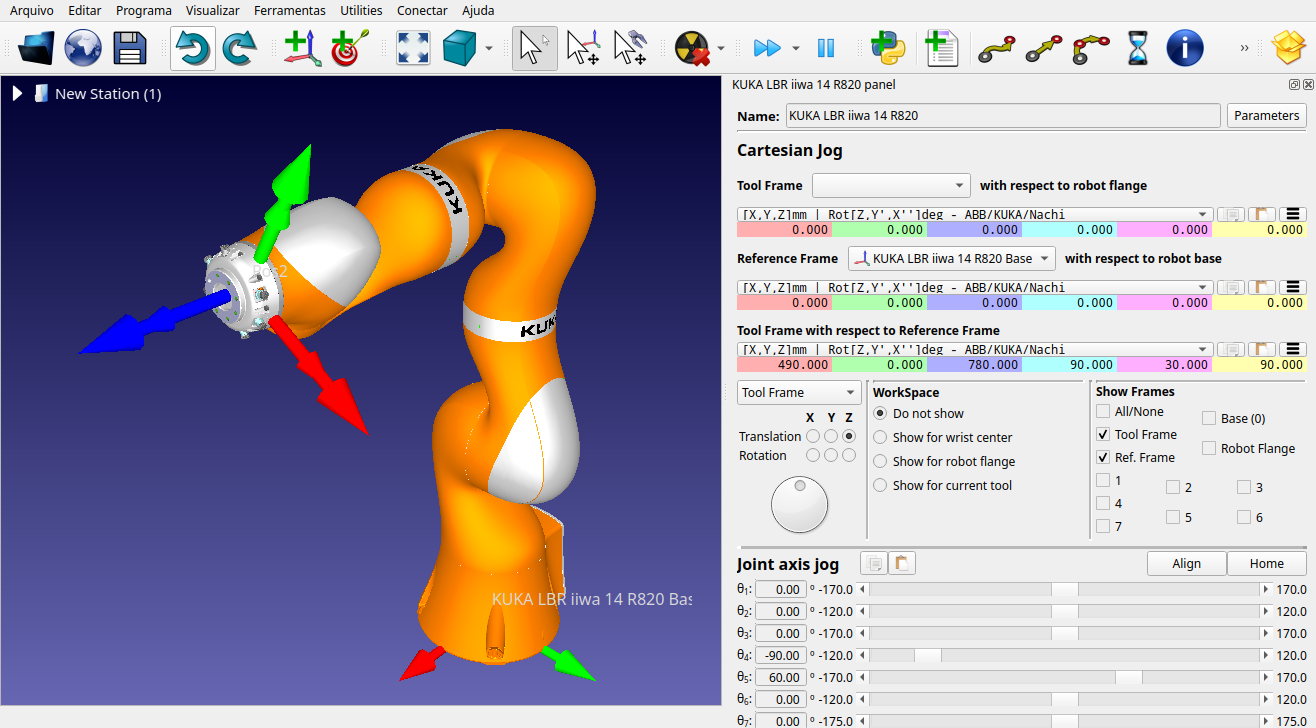
\includegraphics[width=8cm]{Imagem/escolhido.png}
    \caption{Posição escolhida para o robô KUKA LBR iiwa}
    \label{fig:escolhida}
\end{figure}

É possível observar que, do frame zero ao quatro tem-se um a translação de  da pose \textit{home} para a escolhida, ocorreu uma rotação de \ang{60} no link 5 ($\theta_5$) e de $-\ang{90}$ no link 4 ($\theta_4$). Além disso, a translação do frame zero para o sete passa a ser de 78 cm no eixo $z$ e de 49 cm em $x$.

No RoboDK, a pose do \textit{end-effector} é retornada com a translação nos eixos, mas a rotação em $z$, $y'$ e $x''$. Isto é, a composição de rotações no frame atual para os valores indicados.
    
Para a configuração escolhida em $\tt T\_$, são dados
\begin{equation*}
    R_7^0 = \Rot_{z,\,\ang{90}} \Rot_{y,\,\ang{30}} \Rot_{x,\,\ang{90}}
\end{equation*}
Aplicando os valores
\begin{align*}
R = 
\left[ 
\begin{array}{rrr}
    0 & -1 & 0 \\
    1 &  0 & 0 \\
    0 &  0 & 1
\end{array}
\right]
\left[ 
\begin{array}{rrr}
    \sqrt{3}/2 & 0 & 1/2 \\
    0 &  1 & 0 \\
    -1/2 &  0 & \sqrt{3}/2
\end{array}
\right]\left[ 
\begin{array}{rrr}
    1 & 0 &  0 \\
    0 & 0 & -1 \\
    0 & 1 & 0
\end{array}
\right]
\end{align*}
que resultam em
\begin{align}
    R = \left[ 
\begin{array}{rrr}
    0 & 0 & 1 \\
    \sqrt{3}/2 & 1/2 & 0 \\
    -1/2 & \sqrt{3}/2 & 0
\end{array}
\right]
\end{align}

Comparando com a submatriz de rotação em \eqref{eq:Tescolhido} e \eqref{eq:R_validacao}, verifica-se que o resultado encontrado coincide com o obtido no código e na análise dimensional. Novamente, o modelo geométrico do robô obtido teve êxito e foi validado.